\documentclass[a4, 11pt]{article}
\usepackage{hyperref}
\usepackage[toc,page]{appendix}
\usepackage[table,xcdraw]{xcolor}
\usepackage{pgfgantt}
\usepackage{geometry}

 \geometry{
 a4paper,
 left=1in,
 right=1in, 
 top=1.44in,
 bottom=1.44in
 }

\usepackage[english]{babel}
\usepackage[utf8]{inputenc}
\usepackage{csquotes}
\usepackage{graphicx}
\usepackage{subfig}
\usepackage{fancyhdr}
\usepackage{lscape}
\usepackage{enumitem}
\usepackage{fancyvrb}

\pagestyle{fancy}
\fancyhf{}
\lhead{Uppsala University}
\setlength{\headheight}{20pt}
\cfoot{\thepage}
\rfoot{Sweden from the Eye of GDELT}
\renewcommand{\headrulewidth}{0.5pt}
\renewcommand{\footrulewidth}{0.5pt}

\usepackage[backend=biber,sorting=none]{biblatex}
\addbibresource{sources.bib}



\newcommand{\thesistitle}{Sweden from the Eye of GDELT}
\newcommand{\LIF}{}
\newcommand{\quotes}[1]{``#1''}
\newcommand\tab[1][1cm]{\hspace*{#1}}

\usepackage[backend=biber,sorting=none]{biblatex}
\addbibresource{sources.bib}


\begin{document}
\begin{titlepage}

\begin{figure}
   \vspace{0.2in}
   \begin{center}
     
\includegraphics[scale=0.5]{Images/UU_LOGO.png}
   \end{center}
\end{figure}

\thispagestyle{fancy}

\vspace{1in}

\center

\textsc{\large Project in Data Science }

\vspace{0.6in}

\noindent\vspace{0.1in}\makebox[\linewidth]{\rule{\linewidth}{1.2pt}}
\textsc{ \textbf{\large \thesistitle{}}}
\noindent\makebox[\linewidth]{\rule{\linewidth}{1.2pt}}

\vspace{0.5in}

 \begin{minipage}{0.58\textwidth}
    \begin{flushleft}
        \textit{Students:} \\
        Yaser Kaddoura \\
        Mohammad Mustakim Ur Rahman\\
        yaser.kaddoura.3410@student.uu.se \\
        mohammadmustakim.urrahman.5576@student.uu.se \\
    \end{flushleft}
 \end{minipage}
\begin{minipage}{0.38\textwidth}
    \begin{flushright}
    \textit{Supervisor:} \\
    Raazesh Sainudiin \\
    raazesh.sainudiin@math.uu.se
    \end{flushright}
\end{minipage}

\vspace{1.6in}

\textbf{\large Department of Information Technology} \\

\today

\end{titlepage}


\newpage
\begin{abstract}
     The media contains a wealth of knowledge about the world. The Global
     Database of Events, Language and Tone project, known as GDELT, processes the
     media providing a tangible way to consume the news from the perspective of
     researchers. This paper introduces GDELT with its limitation and
     capabilities so that curious researchers can decide if GDELT is a suitable
     tool for their own needs. The experiments show certain specific media coverages for
     Sweden and Norway while using some of the attributes provided by GDELT,
     such as geographic references, Goldstein scale, and CAMEO codes.
    
\end{abstract}
\begin{center}
    \textbf{Keywords:} GDELT, Media, Big Data, Sweden, Visual Analysis
\end{center}
\setcounter{page}{2}
\newpage


\tableofcontents
\newpage

\section{Introduction}

 The global media tries to report all the ``newsworthy'' events in the world so various human sub-populations  
 can stay informed with the ever-changing set of events. Researchers from different disciplines
 try to capture the state of sub-populations for various reasons; thus making the media a
 valuable medium to do their research. The media generates a massive amount of
 data in different formats and thus making it daunting and limiting for researchers to
 use it without having technologies that can handle big data. The GDELT
 project \cite{GDELT}
 makes it possible to take advantage of the knowledge reported in the world
 by processing all kinds of media and generating a simplified view of it through standardised meta-data. Such meta-data makes 
 GDELT an attractive choice for researchers to conduct their research. This
 paper introduces some of the data sets that GDELT provides while conducting
 experiments on them to showcase GDELT's capabilities, limitations, and
 reliability within the limited scope of this project. 

 \section{The GDELT Project}

 There are two versions of GDELT: GDELT 1.0 that started monitoring the English
 documents in 1979, and GDELT 2.0 that started going beyond English sources from 2015 and thereby 
 allowing it to track the entire globe by monitoring Non-English news in over 65
 languages.

 GDELT 2.0 updates every 15 minutes providing three CSV meta-data files for both 
 English and Non-English (so-called ``multi-lingual"): \textit{Global Knowledge Graph} (GKG),
 \textit{Events}, and \textit{Mentions}. 

 GKG is a structured data that provides different meta-data information extracted from the
 source documents, including, published date, locations, entities, and counts. GDELT also
 has its sentiment analysis system providing the tone of the document and Global
 Content Analysis Measures (GCAM) \cite{GCAM} 
 GCAM consists of over 2,300 latent dimensions
 that can be used to do sentiment analysis, such as, assessing the density of
 anxiety, smugness, and passivity, among others. 

 GDELT extracts inferred events while processing the documents by including an entry in
 the events table with a unique identifier for the inferred ID of each such event.

 Each event has at most two actors (A and B) and an event involves an actor A
 acting on actor B. Each event entry provides information about each actor, such as,
 their name, geographic details, ethnicity, religion, and group, among others. 
 For each event, the entry provides its geographic occurrence details, Conflict and Mediation
 Event Observations (CAMEO) code \cite{CAMEO}, 
 a Goldstein scale \cite{Goldstein}, an average tone for the
 text, and more. The events table uses CAMEO codes to represent different
 information for the actors and the event. An event is represented by at most a
 4 digit CAMEO code providing some context of what the event could be with each
 digit. For example, an event with the code 1411 has the first two digits (14)
 representing the root code for ``PROTEST'', the first three digits (141) for
 ``Demonstrate or rally, not specified below'', and finally the whole number
 (1441) representing ``Demonstrate or rally for leadership change''. GDELT might
 represent an event with fewer digits than 4 if the text doesn't provide
 enough information or if GDELT fails to process the information, if any. Each
 event has a Goldstein scale which gives a score from $-10$ to $10$ that attempts to identify 
 an inferred potential impact of the event on the stability of the local geography, say country, so that
 an event that's related to violence between two actors, for instance, would have a negative score, while an event that expresses any cooperation between two actors would have a positive score. 
 Note that the Goldstein scale depends on the event only; in other words, protesting in a
 group of 10 people has the same value as protesting in a group of of 10,000 people. 
 However, counts of people, in such a case for example, is also in the meta-data, if one wants the the number of people involved in an event as either actor to be accounted for.

 The mentions table is a newly added table to the most recent version (GDELT 2.0). 
 It captures how many times an event is mentioned in the source documents containing the ID
 of the event,
 and how confident GDELT is in extracting the event. One way of using this table is to identify 
 the most covered or reported events in the media. Another way would be to figure out which media
 sources are the most active and what they are covering the most and when and where.

 The appendix holds an Entity Relationship (ER) 
 diagram [Figure~\ref{fig:gdelt_datasets}] to
 visualise the data sets and tree representation of a subset of the CAMEO
 taxonomy for the events [Figure~\ref{fig:cameo_taxonomy}].

 The mentions and GKG tables provide the source language for Non-English
 documents and thus make it possible to focus on specific media depending on the
 language. The three tables can be joined together by using the event ID and the
 document's identifier, in other words the URL for the source document.

 \section{Experiments}

 Apache Spark \cite{Spark} is a popular tool for large-scale data analysis, making it our
 choice to process the massive amount of data provided by GDELT. The experiments
 use GDELT 2.0, since our point of interest is in the Non-English media (Swedish
 and Norwegian) for the year 2021. The experiments will concentrate on the
 events that impact society negatively, meaning that we are only considering the
 events with a negative Goldstein scale, while being mindful that the scale is a simple inferred signal that can be interpreted and may not necessarily be an accurate signal of the true negativity of the event. In this project we were more focused on scalable data explorations that can be improved further as we discuss below. 

 \subsection{Events CAMEO taxonomy in Sweden}

 The first experiment shows the media coverage for the events that have negative
 impact, as measured in Goldstein scale, on society using a treemap [Figure~\ref{fig:cameo}]. 
 The most popular events covered by the
 media are ``INVESTIGATE'', ``FIGHT'' and ``DISAPPROVE'' with  3533, 3251, and
 3014 CAMEO codes, respectively. The colour represents the tone of the text in the
 article. The figure shows the top three events only for visualisation clarity.
 Figure~\ref{fig:cameo_full} in the appendix shows the treemap with all such
 events.

\begin{figure}[htbp]
    \centering
    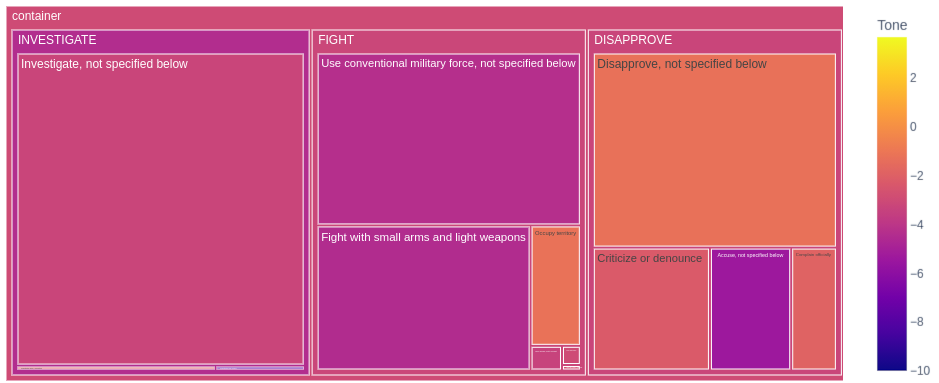
\includegraphics[scale=0.38]{Images/CAMEO.png}%
    \caption{CAMEO events in Sweden} 
    \label{fig:cameo}
\end{figure}

 \subsection{Comparison between Sweden and Norway}

 This experiment compares the Swedish and Norwegian media coverage
 by presenting the moving averages for the coverage of events
 [Figure~\ref{fig:sweden_norway_events}] and their Goldstein scale
 [Figure~\ref{fig:sweden_norway_goldstein}]. The result indicates that the
 Swedish media covers more events than the Norwegian media throughout the year and that significant correlation exists in time between the countries (they rise and fall somewhat together as naturally expected from reports of Scandinavian and global events in both  countries).

\begin{figure}[htbp]
    \centering
    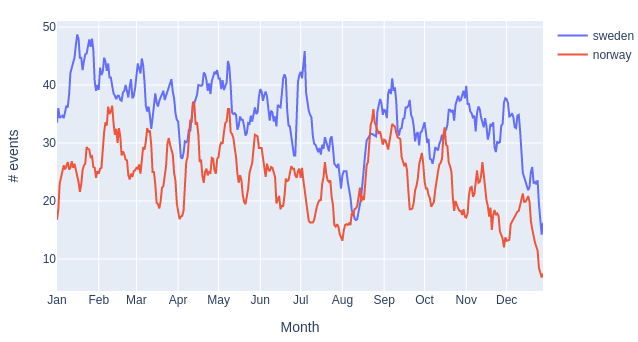
\includegraphics[width=\textwidth]{Images/sweden_norway_events.png}%
    \caption{Events and Godstein scale average in Sweden and Norway for 2021} 
    \label{fig:sweden_norway_events}
\end{figure}

\begin{figure}[htbp]
    \centering
    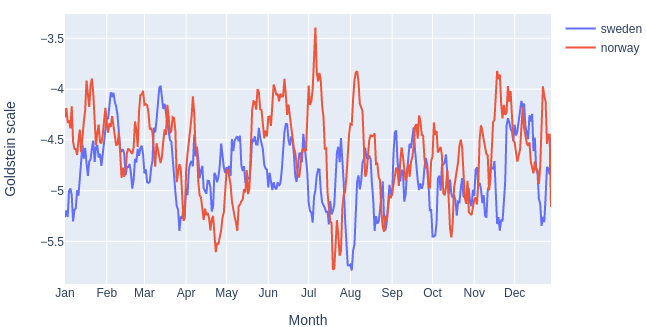
\includegraphics[width=\textwidth]{Images/sweden_norway_goldstein.png}%
    \caption{Events in Sweden and Norway for 2021} 
    \label{fig:sweden_norway_goldstein}
\end{figure}

Figure~\ref{fig:sweden_norway_geo} is a geographic bubble map that shows the coverage of the event for each city. The size of the bubbles represent the number of
events happening inside each city, and the colour represents the average Goldstein
scale. The cities with the most media coverage in both countries are Stockholm, Harjedale, and
Oslo with 2808, 906, and 712, respectively. These figures are instances of the data and the notebooks we provide from this work in \cite{lamastex-gdelt-examples}.
%% leave comment - notebooks will be added here when done editing by raaz in databricks, in time.
%% https://github.com/lamastex/spark-gdelt-examples/tree/master/notebooks/db

\begin{figure}[ht]
    \centering
    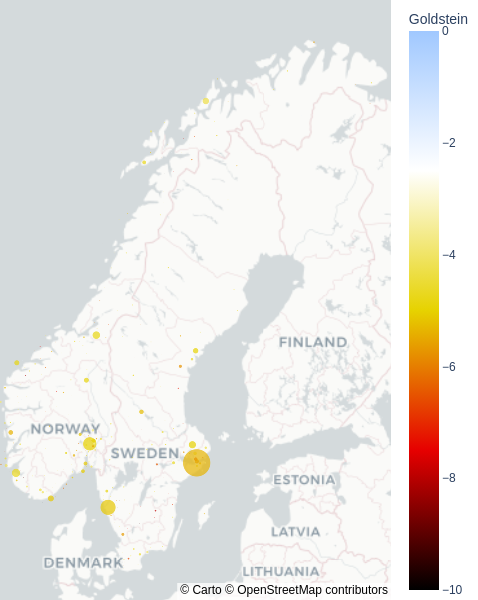
\includegraphics[scale=0.60,angle=90]{Images/sweden_norway_geo.png}
    \caption{Geographic representation of events and Goldstein scale in Sweden and Norway for 2021} 
    \label{fig:sweden_norway_geo}
\end{figure}


 \subsection{Shootings in Sweden}

Crime science is of interest of researchers from different fields who are interested in 
understanding of individual and societal behaviours and structures underpinning criminal 
activities and its effect on the public health. Since crimes can have a major
 effect on the security and sense of well-being of the society it occurs in, 
 it is of paramount interest to quantify the nature and extent of reports of crime-related 
 events in the media. 
 One of the most crucial criminal activity is that committed using firearms. 
 This experimental show-case uses GDELT to extract events related to
 shootings in Sweden from the Swedish media for the year 2021.

 The information provided by GDELT isn't enough to identify shooting
 events. Even though some of the themes that GDELT gives the source articles such as ``KILL''
 and ``ARREST'' have a reasonably good correlation with actual shooting events, they can relate
 to other criminal activities and thus making it a weak choice to extract shooting events. 
 With that said, GDELT can be a good starting point to identify potential articles 
 that mention shooting events.

 The following pipeline identifies if the events mentioned in an article is
 related to shootings:

 \begin{enumerate}
     \item Extract relevant events from GDELT.
     \item Scrape the text of the articles that mention events in step 1.
     \item Translate text to English (unless access to Swedish NLP tools are available). % ok if NLP is explained below now
     \item Perform Natural Language Processing (NLP) techniques to extract terms.
     \item Check if any term related to the shootings from step 4 is present.
 \end{enumerate}

 Using the geographic references provided by GDELT, we can extract the events
 that are happening in Sweden. Instead of processing every event in Sweden, they
 can be limited to the ones that have a negative Goldstein scale, since the
 shooting events harm society. The python package \cite{spacy}
 used to extract the terms from the text did not support the Swedish language at the time of this analysis, so the
 text is machine-translated to English beforehand using \cite{deep-translator}.
 Lastly, the shooting events are
 identified by checking if any of the obtained terms are related to shootings
 such as ``shot'', ``shooting'', or ``gunshots''. We note that there are much more principled ways of doing this NLP pipeline if we have access to GPT3+ models \cite{GPT3} trained directly with a larger Swedish corpus with or without transfer learning and avoiding the machine-translation route using for instance the fastest supercomputer in Sweden \cite{berzelius}. However, such possibilities are outside the scope of this project but possible for future work that build further from our work.

 The time series in figure~\ref{fig:shootings_time_series} shows the number of
 shooting events and mentions for each month covered in the media. The media
 coverage for shooting events peaked in July with 241 events mentioned 378 times
 and October with 205 events mentioned 349 times.

\begin{figure}[htbp]
    \centering
    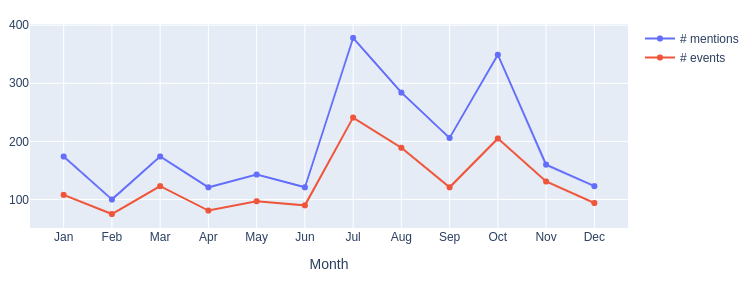
\includegraphics[scale=0.60,angle=0]{Images/sweden_shootings.png}%
    \caption{Media coverage of shootings in Sweden} 
    \label{fig:shootings_time_series}
\end{figure}

 The geographic bubble map in figure~\ref{fig:shootings_geo} indicates the
 number of shooting events in Swedish cities where the cities with the highest
 shooting counts are Stockholm, Harjedale, and Goteborg with 568, 425, and 194, respectively.

\begin{figure}[htbp]
    \centering
    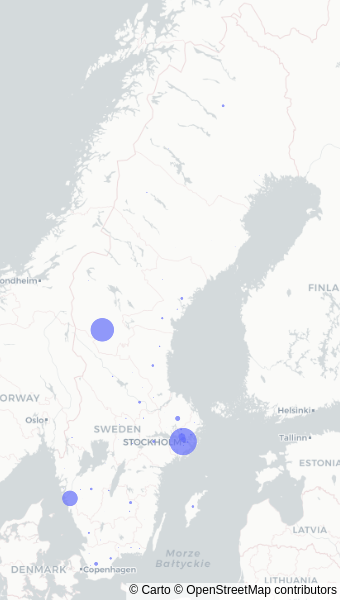
\includegraphics[scale=0.65,angle=90]{Images/shootings_geo.png}%
    \caption{Media coverage of shootings in Swedish cities} 
    \label{fig:shootings_geo}
\end{figure}

\subsection{Reliability}

GDELT is an ambitious project trying to process the entire media. As a
result, the pipelines that it uses produce some noise such as generating more
than one event entry for the same event extracted from different source documents. It
can also generate nonsensical values for the attributes in the events table. 
For example, one GKG entry has a 2 billion count for ``KILL'' which means that 2 billion 
people died because of the event. 

Another example is an erroneous extraction of firearms events from
articles that discuss COVID shots. 
Part of the problem with the ``trans-lingual'' version of GDELT 2.0, is that it already does machine translation of the original Swedish language sources to determine the meta-data. 
Nonetheless, using more careful pipelines that further filter out such bad examples by directly using the source URLs in Swedish using custom-trained Swedish language models is possible, especially by using our scalable scraping framework using goose library implemented in the gdelt library \cite{lamastex-spark-gdelt} we have used in the project to turn the raw GDELT meta-data from CSV files to delta lakes \cite{delta_io}.


\section{Discussion and Future Work}

This paper discussed three of the most common data sets generated by GDELT while
experimenting on them to show their limitation and capabilities. We have emphasised a few bad examples here from a cautionary analytic point of view -- our main objective in this project -- so as to warn researchers that the naive exploratory pipeline developed here should not be directly used without further filtering and cross-examination from the scraped original source articles using NLP tools ideally developed in the original language of the article using a large corpus. We have not had the time and resources (none of us are Swedish speakers, for instance) to identify what fraction of events are mapped to nonsensical values, as such an endeavour is beyond the scope of this project. However, the GDELT signals are still very meaningful in many cases and GDELT is used in practice with success in finance and intelligence domain as a data source for Open Source Intelligence \cite{OSINT}. Moreover, its parent project Google JigSaw \cite{jigsaw} that has had remarkable success in helping make the internet safer, including successful social-media intervention operations done by ``fringe'' or ``radical'' groups from the perspective of State actors. 
Nonetheless, it could be a starting point. It's worth investigating from the
perspective of a researcher interested in social sciences and building NLP
pipelines {\em on top} of what GDELT provides as a stepping stone to achieving
satisfactory results. Building these pipelines will require one to have a background
or the will to spend time learning some technologies that are related to big
data and NLP, but it will be worth the while from a researcher's point of view,
especially in this era. If clean and reliable data related to the topic of
research isn't available, then GDELT is the best bet, especially by considering the remarks we made regarding the use of Swedish-specific Open AI models like GPT3. 

In order to perform a more thorough interpretation of the results and help dive deeper from our current project work which itself build on previous projects, our project is available as examples and notebooks at \cite{lamastex-gdelt-examples}. 
\section{Acknowledgements}

This project was supported by {\em Combient Mix AB} through a {\em Data Science Project Fellowships} between 2021-10 and 2021-12 to Yaser Kaddoura and Mohammad Mustakim Ur Rahman at {\em Combient Competence Centre for Data Engineering Sciences}, Department of Mathematics, Uppsala University, Uppsala, Sweden, and {\em Databricks University Alliance} with infrastructure credits from {\em AWS} to Raazesh Sainudiin, Department of Mathematics, Uppsala University, Sweden. Many thanks to Andrew Morgan and Antoine Amend for their guidance.

\newpage

\begin{appendices}

\section{About GDELT}

\subsection{Some GDELT data sets}

The ER diagram presented in Figure~\ref{fig:gdelt_datasets} shows three of the
most common data sets generated by GDELT.

\begin{figure}[ht] 
    \centering
    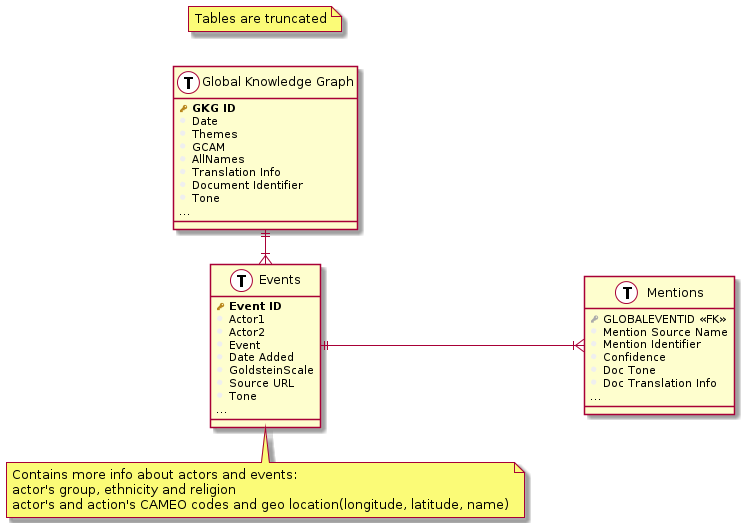
\includegraphics[width=\textwidth]{Images/gdelt_datasets.png}%
    \caption{Some data sets in GDELT} 
    \label{fig:gdelt_datasets}
\end{figure}

\subsection{CAMEO events taxonomy}

The tree in Figure~\ref{fig:cameo_taxonomy} represents a subset of the taxonomy
for CAMEO events. The children nodes add more context to the events presented by
their parents.

\begin{figure}[ht]
    \centering
    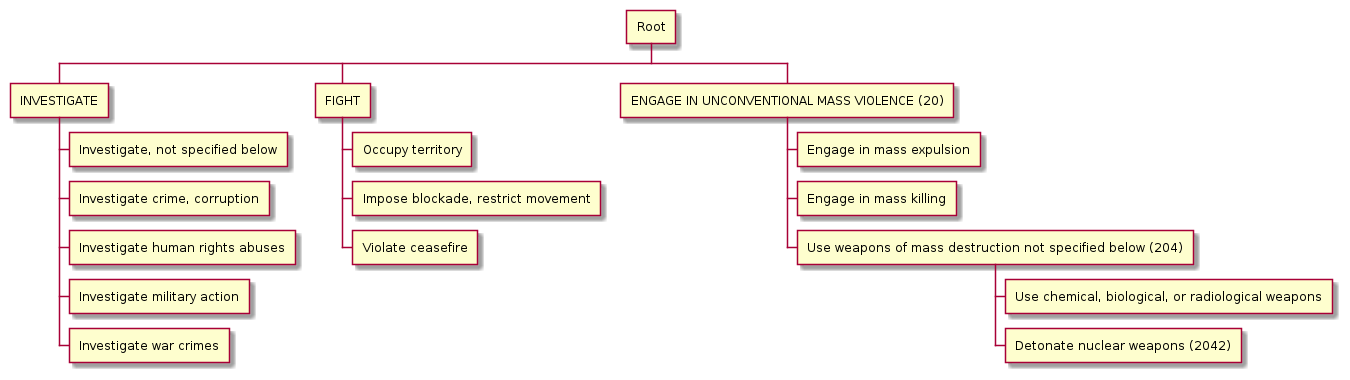
\includegraphics[scale=0.3]{Images/CAMEO_taxonomy.png}%
    \caption{A subset of CAMEO events taxonomy} 
    \label{fig:cameo_taxonomy}
\end{figure}

\section{Experiments}
\subsection{Every event for CAMEO experiment}

Figure \ref{fig:cameo_full} is the full version of the treemap for the events
in Sweden. Notice that the events related to ``Sexual assault'' and ``Arrest, detain,
or charge with legal actions'' have the lowest tone.

\begin{figure}[ht]
    \centering
    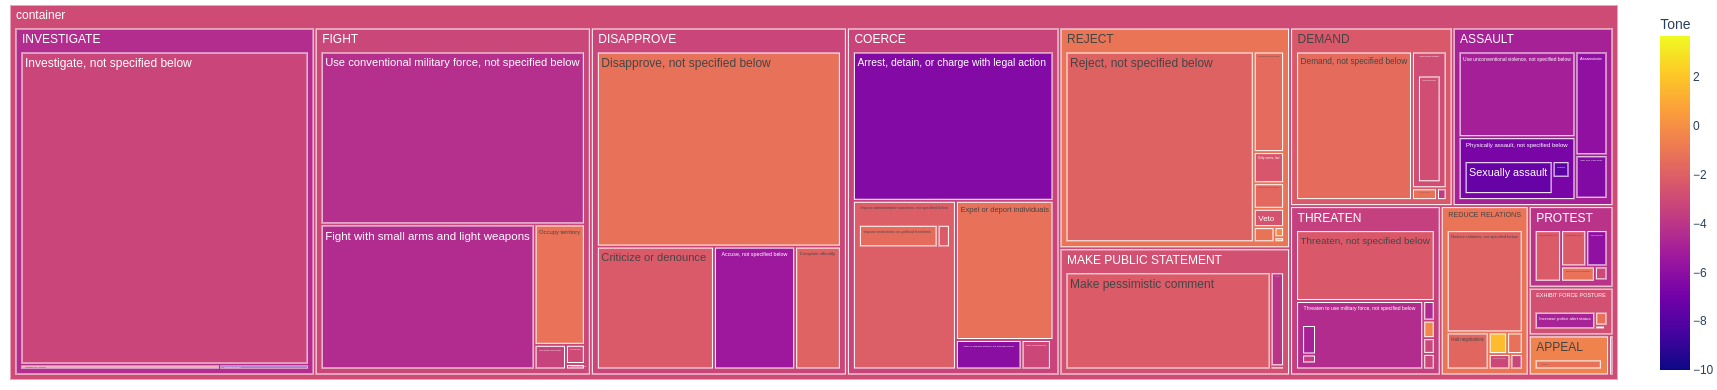
\includegraphics[scale=0.25]{Images/CAMEO_full.png}%
    \caption{CAMEO events in Sweden (Full version)} 
    \label{fig:cameo_full}
\end{figure}

\end{appendices}

\nocite{*}
\printbibliography

\end{document}
